\documentclass{article}

\usepackage[margin=0.5in]{geometry}
\usepackage{multicol}
\usepackage{siunitx}
\usepackage{enumitem}
\usepackage{graphicx}
\usepackage{amsthm}
\usepackage{amsmath}

\title{Polygons Homework}
\author{}
\date{}

\begin{document}
\maketitle
\section*{Polygon Angles}
The sum of the interior angles of a polygon with $n$ sides is $180(n - 2)$. 
Exterior angles in a polygon always sum up to $\ang{360}$.
\begin{enumerate}
    \item If $\angle A = \ang{20}$ and $\angle AFG = \angle AGF$, then what is $\angle B + \angle D$?
        \begin{center}
            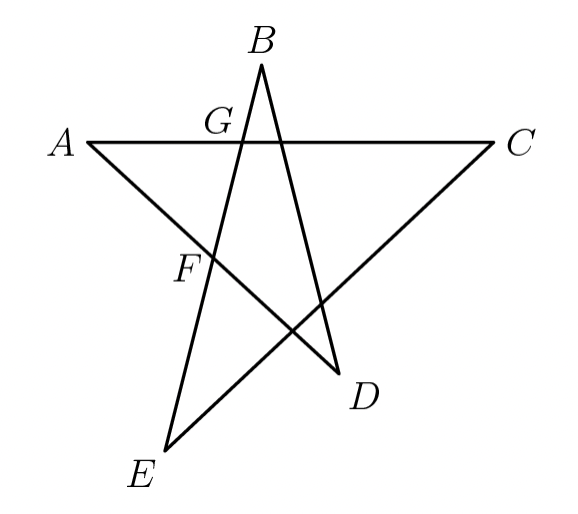
\includegraphics[scale=0.5]{star.png}
        \end{center}
        \vspace{1cm}
    \item What is the interior angle measure of a regular $15$-agon?
        \vspace{3cm}
    \item A polygon has $11$ sides and $10$ congruent $\ang{150}$ interior angles.
        What is the measure of its largest exterior angle?
        \vspace{3 cm}
\end{enumerate}

\section*{Trapezoids}
\begin{enumerate}[resume]
    \item In trapezoid $ABCD$, the sides $AB$ and $CD$ are equal. 
        What is the perimeter of $ABCD$?
        \begin{center}
            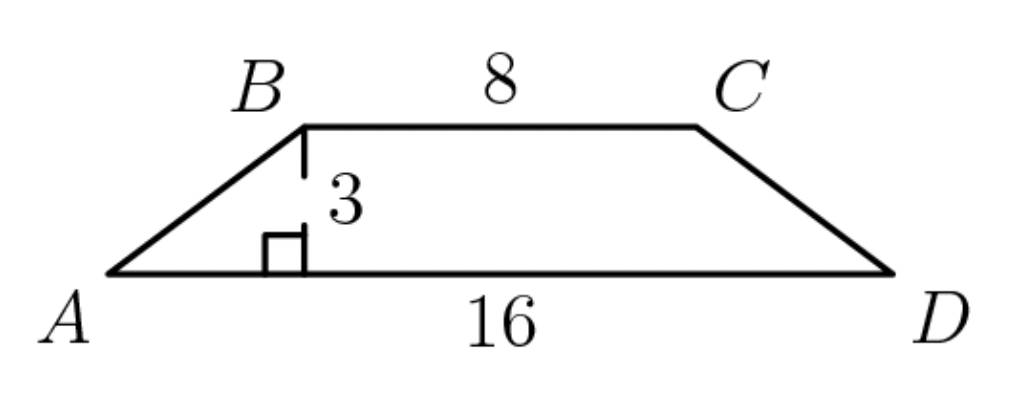
\includegraphics[scale=0.4]{trapezoid1.png}
        \end{center}
        \vspace{3cm}
\end{enumerate}

\section*{Parallelograms}
\begin{enumerate}[resume]
    \item In parallelogram $ABCD$, diagonals $AC$ and $BD$ intersect at $E$.
        If $AE = 2x + 9$ and $CE = 5x$, what is the length of diagonal $AC$?
        \vspace{3cm}
    \item In parallelogram $ABCD$, diagonal $AC$ is twice the length of diagonal $BD$.
        The perimeter of triangle $ABC$ is $21$ cm and the perimeter of triangle $BCD$ is $17$ cm.
        What is the perimeter of parallelogram $ABCD$?
        \vspace{3cm}
\end{enumerate}
\end{document}
